%
% file : descrption.tex
% date : samedi 11 janvier 2020, 12:24:22 (UTC+0100)
% author : sedelpeuch
% description :
\documentclass[a4paper,10pt]{report}
\usepackage[utf8]{inputenc}
\usepackage[T1]{fontenc}
\usepackage[french]{babel}
\usepackage{graphicx}
\usepackage{ulem}
\usepackage{float}
\usepackage{amsmath}
\usepackage{amssymb}
\usepackage{mathrsfs}
\usepackage{color}
\usepackage{fancyhdr}
\usepackage{pdfpages}
\usepackage{layout}
\usepackage{multicol}
\usepackage{setspace}
\usepackage{tabularx,array}
\usepackage[colorlinks=true]{hyperref}
\usepackage{tikz, tkz-tab}
\usepackage[top=2cm,bottom=2cm,left=2cm,right=2cm]{geometry}
\usepackage{amsthm}
\usepackage{listings}
\setlength{\parindent}{1cm}
\setlength{\parskip}{1ex plus 0.5ex minus 0.2ex}
\newcommand{\hsp}{\hspace{20pt}}
\newcommand{\HRule}{\rule{\linewidth}{0.5mm}}


\begin{document}
\begin{spacing}{1.5}
\graphicspath{{../reunion/}}
\begin{titlepage}
\begin{sffamily}
\begin{center}
\vspace*{\stretch{1}}
\textsc{\LARGE Eirbot \\ Coupe de France de robotique}\\[2cm]
\HRule \\[0.4cm]
{\huge \bfseries Equipe Eirboat \\[0.4cm]}

\HRule \\[2cm]

\textsc{\Large 1A 2019-2020}\\[2cm]
              
\includegraphics[scale=0.3]{LogoEirbot.png} \vfill

\vspace*{\stretch{1}}
  \end{center}
  \end{sffamily}
\end{titlepage}
\setcounter{tocdepth}{2}
\tableofcontents
\newpage
\pagestyle{fancy}
\lhead{}
\chead{\textbf{}}
\rhead{\thepage}
\lfoot{}
\cfoot{}
 \fancyfoot[R]
 {
 
\includegraphics[scale=0.075]{65508.png}
 }

 \setcounter{part}{1}
\part{Description des projets}
\chapter{Description générale de l'organisation}
\section{Arbres des tâches à réaliser par le robot}
\label{taches}
\HRule
\begin{center}
\begin{tikzpicture}
\tikzstyle{lien}=[->,>=stealth,rounded corners=20pt,thick]
\tikzset{individu/.style={draw,thick,fill=#1!25},
individu/.default={white}}
\node[individu=blue] (A) at (0,0) {\textsc{Se mouvoir}};
\node[individu] (A1) at (-7,-2) {Odométrie};
\node[individu] (A2) at (-3,-2) {Moteurs Maxon};
\node[individu] (A3) at (7,-2) {Asservissement};
\node[individu] (A3b) at (7,-4) {Encodeur};
\node[individu] (A4) at (3,-2) {\xout{Roue folle 2 roues motrices}};
\node[individu] (A5) at (3,-4) {2 roues motrice + patins};

\draw[lien] (A) -- (A1);
\draw[lien] (A) -- (A2);
\draw[lien] (A) -- (A3);
\draw[lien] (A) -- (A4);
\draw[lien] (A3) -- (A3b);
\draw[lien] (A4) -- (A5);


\end{tikzpicture}
\end{center}

\begin{center}
\begin{tikzpicture}
\tikzstyle{lien}=[->,>=stealth,rounded corners=20pt,thick]
\tikzset{individu/.style={draw,thick,fill=#1!25},
individu/.default={white}}
\node[individu=blue] (A) at (0,0) {\textsc{Mécanique générale}};
\node[individu] (A1) at (-3,-2) {Structure octogonale};
\node[individu] (A2) at (0,-2) {Profilés};
\node[individu] (A3) at (3,-2) {Etage rectangulaire};

\draw[lien] (A) -- (A1);
\draw[lien] (A) -- (A3);
\draw[lien] (A) -- (A2);

\end{tikzpicture}
\end{center}
\HRule
\begin{multicols}{2}
\begin{center}
\begin{tikzpicture}
\tikzstyle{lien}=[->,>=stealth,rounded corners=20pt,thick]
\tikzset{individu/.style={draw,thick,fill=#1!25},
individu/.default={white}}
\node[individu=red] (A) at (0,0) {\textsc{Détecter adversaire}};
\node[individu] (A1) at (0,-2) {Capteurs};
\node[individu] (A1a) at (-2,-4) {\xout{Ultrasons}};
\node[individu] (A1b) at (2,-4) {Infra rouge};

\draw[lien] (A) -- (A1);
\draw[lien] (A1) -- (A1a);
\draw[lien] (A1) -- (A1b);

\end{tikzpicture}
\end{center}
\columnbreak
\begin{center}
\begin{tikzpicture}
\tikzstyle{lien}=[->,>=stealth,rounded corners=20pt,thick]
\tikzset{individu/.style={draw,thick,fill=#1!25},
individu/.default={white}}
\node[individu=red] (A) at (0,0) {\textsc{Détecter Objet}};
\node[individu] (A1) at (-2,-2) {Couleur écocup};
\node[individu] (A1a) at (-2,-4) {Capteurs RGB};\node[individu] (A2) at (2,-2) {Pendant le ramassage};

\draw[lien] (A) -- (A1);
\draw[lien] (A1) -- (A1a);
\draw[lien] (A) -- (A2);
\draw (-3,0) -- (3,-4);
\draw (3,0) -- (-3,-4);


\end{tikzpicture}
\end{center}
\end{multicols}

\begin{multicols}{2}
\begin{center}
\begin{tikzpicture}
\tikzstyle{lien}=[->,>=stealth,rounded corners=20pt,thick]
\tikzset{individu/.style={draw,thick,fill=#1!25},
individu/.default={white}}
\node[individu=red] (A) at (0,0) {\textsc{Lire boussole}};
\node[individu] (A1) at (-2,-2) {Capteur};
\node[individu] (A1a) at (-2,-4) {Webcam};\node[individu] (A2) at (2,-2) {Balise sur le côté};

\draw[lien] (A) -- (A1);
\draw[lien] (A1) -- (A1a);
\draw[lien] (A) -- (A2);

\end{tikzpicture}
\end{center}
\columnbreak
\begin{center}
\begin{tikzpicture}
\tikzstyle{lien}=[->,>=stealth,rounded corners=20pt,thick]
\tikzset{individu/.style={draw,thick,fill=#1!25},
individu/.default={white}}
\node[individu=red] (A) at (0,0) {\textsc{Communication}};
\node[individu] (A1) at (-2,-2) {InfraRouge};;\node[individu] (A2) at (2,-2) {Bluetooth};

\draw[lien] (A) -- (A1);
\draw[lien] (A) -- (A2);

\end{tikzpicture}
\end{center}
\end{multicols}
\HRule

\begin{multicols}{2}
\begin{center}
\begin{tikzpicture}
\tikzstyle{lien}=[->,>=stealth,rounded corners=20pt,thick]
\tikzset{individu/.style={draw,thick,fill=#1!25},
individu/.default={white}}
\node[individu=green] (A) at (0,0) {\textsc{Elévation drapeau}};
\node[individu] (A1) at (-2,-2) {Timer};
\node[individu] (A2) at (2,-2) {Servomoteurs};

\draw[lien] (A) -- (A1);
\draw[lien] (A) -- (A2);

\end{tikzpicture}
\end{center}
\columnbreak
\begin{center}
\begin{tikzpicture}
\tikzstyle{lien}=[->,>=stealth,rounded corners=20pt,thick]
\tikzset{individu/.style={draw,thick,fill=#1!25},
individu/.default={white}}
\node[individu=green] (A) at (0,0) {\textsc{Manche à air}};
\node[individu] (A1) at (-2,-2) {Servomoteurs};
\node[individu] (A2) at (2,-2) {Coupler activation phare};

\draw[lien] (A) -- (A1);
\draw[lien] (A) -- (A2);

\end{tikzpicture}
\end{center}
\end{multicols}
\HRule

\begin{center}
\begin{tikzpicture}
\tikzstyle{lien}=[->,>=stealth,rounded corners=20pt,thick]
\tikzset{individu/.style={draw,thick,fill=#1!25},
individu/.default={white}}
\node[individu=gray] (A) at (0,0) {\textsc{Cartes}};
\node[individu] (A1) at (-4,-2) {Carte de puissance};
\node[individu] (A2) at (0,-2) {Carte de sécurité};
\node[individu] (A3) at (4,-2) {Carte d'alimentation};

\draw[lien] (A) -- (A1);
\draw[lien] (A) -- (A2);
\draw[lien] (A) -- (A3);


\end{tikzpicture}
\end{center}
\HRule

\begin{center}
\begin{tikzpicture}
\tikzstyle{lien}=[->,>=stealth,rounded corners=20pt,thick]
\tikzset{individu/.style={draw,thick,fill=#1!25},
individu/.default={white}}
\node[individu=orange] (A) at (0,0) {\textsc{Phare}};
\node[individu] (A1) at (-6,-2) {Elévation};
\node[individu] (A1a) at (-8,-4) {Bras robot};
\node[individu] (A1b) at (-4,-4) {\xout{Crémaillère}};
\node[individu] (A2) at (0,-2) {Activation};
\node[individu] (A2a) at (-1,-4) {\xout{Ddp}};
\node[individu] (A2b) at (1,-4) {Boutons};
\node[individu] (A3) at (6,-2) {Lumière};
\node[individu] (A3a) at (5,-4) {Ruban LED};
\node[individu] (A3b) at (7,-4) {\xout{Projo}};

\draw[lien] (A) -- (A1);
\draw[lien] (A1) -- (A1a);
\draw[lien] (A1) -- (A1b);
\draw[lien] (A) -- (A2);
\draw[lien] (A2) -- (A2a);
\draw[lien] (A2) -- (A2b);
\draw[lien] (A) -- (A3);
\draw[lien] (A3) -- (A3a);
\draw[lien] (A3) -- (A3b);


\end{tikzpicture}
\end{center}
\HRule

\newpage
\section{Répartition des tâches}
\label{repartition}
\HRule
\begin{center}
\begin{tikzpicture}
\tikzstyle{lien}=[->,>=stealth,rounded corners=20pt,thick]
\tikzset{individu/.style={draw,thick,fill=#1!25},
individu/.default={white}}
\node[individu=blue] (A) at (0,0) {\textsc{Se mouvoir} Carte puissance};
\node[individu] (A1) at (-3,-2) {Martin};
\node[individu] (A2) at (-1,-2) {\xout{Julien}};
\node[individu] (A3) at (1,-2) {Valentin};
\node[individu] (A4) at (3,-2) {Filipe};

\draw[lien] (A) -- (A1);
\draw[lien] (A) -- (A2);
\draw[lien] (A) -- (A3);
\draw[lien] (A) -- (A4);


\end{tikzpicture}
\end{center}
\begin{center}
\begin{tikzpicture}
\tikzstyle{lien}=[->,>=stealth,rounded corners=20pt,thick]
\tikzset{individu/.style={draw,thick,fill=#1!25},
individu/.default={white}}
\node[individu=blue] (A) at (0,0) {\textsc{Se mouvoir} Odométrie \& Asservissement};
\node[individu] (A1) at (-5,-2) {\xout{Raphaël}};
\node[individu] (A2) at (0,-2) {Clément};
\node[individu] (A3) at (5,-2) {SD};
\node[individu] (A4) at (-3,-2) {Emile};
\node[individu] (A5) at (3,-2) {Liam};

\draw[lien] (A) -- (A1);
\draw[lien] (A) -- (A2);
\draw[lien] (A) -- (A3);
\draw[lien] (A) -- (A4);
\draw[lien] (A) -- (A5);

\end{tikzpicture}
\end{center}

\begin{center}
\begin{tikzpicture}
\tikzstyle{lien}=[->,>=stealth,rounded corners=20pt,thick]
\tikzset{individu/.style={draw,thick,fill=#1!25},
individu/.default={white}}
\node[individu=blue] (A) at (0,0) {\textsc{Mécanique Générale}};
\node[individu] (A1) at (-4,-2) {Erwann};
\node[individu] (A2) at (-2,-2) {Julien};
\node[individu] (A3) at (2,-2) {\xout{Valentin}};
\node[individu] (A4) at (4,-2) {\xout{Marion}};

\draw[lien] (A) -- (A1);
\draw[lien] (A) -- (A2);
\draw[lien] (A) -- (A3);
\draw[lien] (A) -- (A4);

\end{tikzpicture}
\end{center}
\HRule
\begin{multicols}{2}
\begin{center}
\begin{tikzpicture}
\tikzstyle{lien}=[->,>=stealth,rounded corners=20pt,thick]
\tikzset{individu/.style={draw,thick,fill=#1!25},
individu/.default={white}}
\node[individu=red] (A) at (0,0) {\textsc{Détecter Adversaire}};
\node[individu] (A1) at (-4,-2) {Martin};
\node[individu] (A2) at (-2,-2) {Liam};
\node[individu] (A3) at (2,-2) {\xout{Jeremy}};
\node[individu] (A4) at (4,-2) {\xout{Raphaël}};

\draw[lien] (A) -- (A1);
\draw[lien] (A) -- (A2);
\draw[lien] (A) -- (A3);
\draw[lien] (A) -- (A4);

\end{tikzpicture}
\end{center}
\columnbreak
\begin{center}
\begin{tikzpicture}
\tikzstyle{lien}=[->,>=stealth,rounded corners=20pt,thick]
\tikzset{individu/.style={draw,thick,fill=#1!25},
individu/.default={white}}
\node[individu=red] (A) at (0,0) {\textsc{Lire boussole}};
\node[individu] (A1) at (-2,-2) {Maxime};
\node[individu] (A2) at (0,-2) {Emile};
\node[individu] (A3) at (2,-2) {Léo};

\draw[lien] (A) -- (A1);
\draw[lien] (A) -- (A2);
\draw[lien] (A) -- (A3);

\end{tikzpicture}
\end{center}
\end{multicols}
\HRule
\begin{multicols}{2}
\begin{center}
\begin{tikzpicture}
\tikzstyle{lien}=[->,>=stealth,rounded corners=20pt,thick]
\tikzset{individu/.style={draw,thick,fill=#1!25},
individu/.default={white}}
\node[individu=green] (A) at (0,0) {\textsc{Elévation drapeau}};
\node[individu] (A1) at (-3,-2) {Filipe};
\node[individu] (A2) at (3,-2) {Erwann};
\node[individu] (A3) at (0,-2) {Valentin};

\draw[lien] (A) -- (A1);
\draw[lien] (A) -- (A2);
\draw[lien] (A) -- (A3);

\end{tikzpicture}
\end{center}
\columnbreak
\begin{center}
\begin{tikzpicture}
\tikzstyle{lien}=[->,>=stealth,rounded corners=20pt,thick]
\tikzset{individu/.style={draw,thick,fill=#1!25},
individu/.default={white}}
\node[individu=green] (A) at (0,0) {\textsc{Manche à air}};
\node[individu] (A1) at (-3,-2) {\xout{Jeremy}};
\node[individu] (A2) at (3,-2) {Marius};
\node[individu] (A3) at (0,-2) {Filipe};

\draw[lien] (A) -- (A1);
\draw[lien] (A) -- (A2);
\draw[lien] (A) -- (A3);

\end{tikzpicture}
\end{center}
\end{multicols}
\HRule

\begin{center}
\begin{tikzpicture}
\tikzstyle{lien}=[->,>=stealth,rounded corners=20pt,thick]
\tikzset{individu/.style={draw,thick,fill=#1!25},
individu/.default={white}}
\node[individu=orange] (A) at (0,0) {\textsc{Phare}};
\node[individu] (A1) at (-4,-2) {\xout{Marion}};
\node[individu] (A2) at (-2,-2) {\xout{Jeremy}};
\node[individu] (A3) at (2,-2) {Marius};
\node[individu] (A4) at (4,-2) {\xout{Erwann}};

\draw[lien] (A) -- (A1);
\draw[lien] (A) -- (A2);
\draw[lien] (A) -- (A3);
\draw[lien] (A) -- (A4);

\end{tikzpicture}
\end{center}
\HRule

\begin{center}
\begin{tikzpicture}
\tikzstyle{lien}=[->,>=stealth,rounded corners=20pt,thick]
\tikzset{individu/.style={draw,thick,fill=#1!25},
individu/.default={white}}
\node[individu=gray] (A) at (0,0) {\textsc{Alimentation}};
\node[individu] (A1) at (-3,-2) {Julien};
\node[individu] (A2) at (-0,-2) {Ptit Lu};
\node[individu] (A3) at (3,-2) {Yohann};
\node[individu] (A4) at (5,-2) {\xout{Théo}};
\node[individu] (A5) at (-5,-2) {Léo};

\draw[lien] (A) -- (A1);
\draw[lien] (A) -- (A2);
\draw[lien] (A) -- (A3);
\draw[lien] (A) -- (A4);
\draw[lien] (A) -- (A5);

\end{tikzpicture}
\end{center}
\HRule

\section{Points pour la coupe}
\begin{center}
\begin{tikzpicture}
\tikzstyle{lien}=[->,>=stealth,rounded corners=20pt,thick]
\tikzset{individu/.style={draw,thick,fill=#1!25},
individu/.default={white}}
\node[individu=blue] (A) at (0,0 ){\textsc{Bouées}};
\node[individu] (A1) at (5,2){4 pour l'équipe à proximité du ports};
\node[individu] (A2) at (5,1){8 communs directement sur la table};
\node[individu] (A3) at (5,-1){6 pour l'équipe dans un ecceuil};
\node[individu] (A4) at (5,-2){12 communs dans des ecceuils};


\draw[lien] (A) --(0,2)-- (A1);
\draw[lien] (A) --(0,1)-- (A2);
\draw[lien] (A) --(0,-1)-- (A3);
\draw[lien] (A) --(0,-2)-- (A4);

\node[individu] (A5) at (-5,1){1 points par bouée valide};
\node[individu] (A6) at (-5,0){1 sup si la bouée est sur le bon chenal};
\node[individu] (A7) at (-5,-1){2 points par paire de bouée};


\draw[lien] (A) --(0,1)-- (A5);
\draw[lien] (A) -- (A6);
\draw[lien] (A) --(0,-1)-- (A7);

\tikzstyle{lien}=[->,>=stealth,rounded corners=20pt,thick]
\tikzset{individu/.style={draw,thick,fill=#1!25},
individu/.default={white}}
\node[individu=red] (B) at (0,-5 ){\textsc{Manche à air}};
\node[individu] (B1) at (5,-5){2 manche à airs au Sud du port};
\draw[lien] (B) -- (B1);


\node[individu] (B5) at (-5,-4){5 pour 1 manche};
\node[individu] (B6) at (-5,-6){15 pour 2 manches};


\draw[lien] (B) --(0,-4)-- (B5);
\draw[lien] (B) -- (0,-6) -- (B6);

\tikzstyle{lien}=[->,>=stealth,rounded corners=20pt,thick]
\tikzset{individu/.style={draw,thick,fill=#1!25},
individu/.default={white}}
\node[individu=green] (C) at (0,-10 ){\textsc{Allumer le phare}};
\node[individu] (C1) at (5,-10){1 phare au nord du port};
\draw[lien] (C) -- (C1);


\node[individu] (C5) at (-5,-9){2 pour poser le phare};
\node[individu] (C6) at (-5,-10){3 pour le déclancher};
\node[individu] (C7) at (-5,-11){10 pour activation correcte};


\draw[lien] (C) --(0,-9)-- (C5);
\draw[lien] (C) -- (0,-11) -- (C7);
\draw[lien] (C) -- (C6);

\node[individu=yellow] (D) at (0,-15 ){\textsc{Retourner au port}};
\node[individu] (D1) at (5,-15){Sur les largeurs de la table};
\draw[lien] (D) -- (D1);


\node[individu] (D5) at (-5,-13){1 robot 10 dans la bonne zone};
\node[individu] (D6) at (-5,-14){1 robot 5 dans la mauvaise zone};
\node[individu] (D7) at (-5,-16){2 robots 10 dans la bonne zone};
\node[individu] (D8) at (-5,-17){2 robots 5 dans la mauvaise zone};
\node[individu] (D9) at (-5,-18){2 robots 5 1 dans la bonne zone};
\node[individu] (D10) at (-5,-19){2 robots 5 dans des zones différentes};


\draw[lien] (D) --(0,-13)-- (D5);
\draw[lien] (D) --(0,-14)-- (D6);
\draw[lien] (D) -- (0,-16) -- (D7);
\draw[lien] (D) -- (0,-17) -- (D8);
\draw[lien] (D) -- (0,-18) -- (D9);
\draw[lien] (D) -- (0,-19) -- (D10);
\end{tikzpicture}
\end{center}

\chapter{Mécanique}
\section{Mécanique générale du robot}
\section{Actionneurs}

\chapter{Electronique}
\section{Alimentation}
\paragraph{Objectif.} La carte d'alimentation doit distribuer l'énergie et
convertir les tensions. Elle récupère l'énergie de la batterie et elle possède
les caractéristiques suivantes :
\begin{itemize}
\item Moteurs : 3A/moteurs
\item Logique 5V 1.5A
\item Puissance 5V 3A
\item Puissance 12V 3A
\end{itemize}
\begin{figure}[H]
  \center
  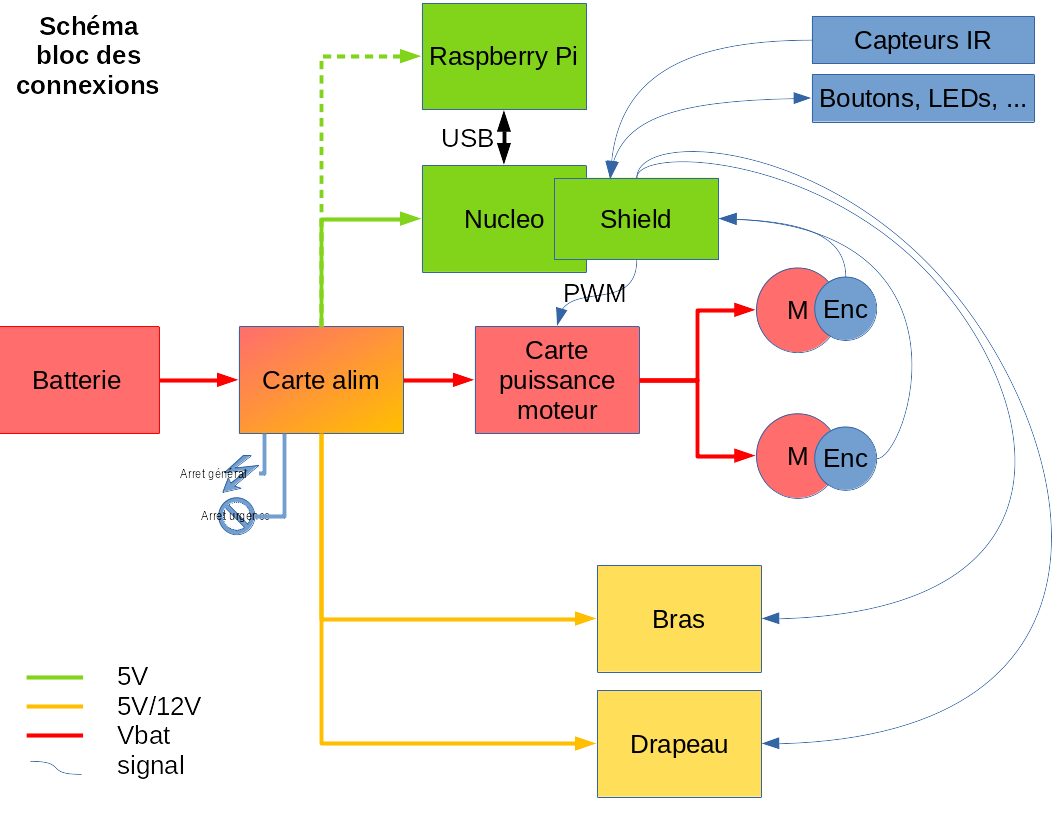
\includegraphics[scale=0.4]{schema_bloc_connexions.png}
\end{figure}
Les détails techniques sont disponibles dans le dossier
\href{https://github.com/eirbot/eirbot2020-1A/tree/master/alim}{alimentation}
sur github.
\section{Puissance}
\section{Actionneur}

\chapter{Informatique}
\section{Asservissement}
\section{Stratégie}
\subsection{Modélisation de la table - Définition des obstacles}
\paragraph{Objectif.} Cette section de la stratégie est la première section,
elle a pour but de définir l'environnement dans lequel le robot va évoluer.
Cette définition de l'environnement sera cruciale pour la recherche de chemin.
L'objectif est donc de créer un système permettant de définir des obstacles et
des méthodes permettant de verifier si il y a des obstacles à un endroit.

\paragraph{Définition d'un obstacle.} La structure permettant de définir un
obstacle est relativement simple, elle contient la position du centre d'un
obstacle, sa largeur et sa longueur. Avec cette définition tous nos obstacles
sont rectangulaires. Par la suite, nous avons renseigné les positions de tous
les obstacles et leurs types (eco cup, petit taquet, grand taquet). Nous mettons
toutes ces informations dans un vecteur. Ce vecteur sera l'élément de base pour
détecter les collisions entre notre robot et les obstacles.

\paragraph{Prévision de collision.} L'idée est d'obtenir une méthode permettant
de savoir si notre robot peut aller à un point donné sans toucher d'obstacles.
Nous réalisons un test mathématique simple qui permet de nous donner en fonction
de coordonées $x,y$, d'une forme d'obstacle et d'une liste contenant tous les
obstacles si la case est valide ou non. Le fait de pouvoir tester les
différentes formes d'obstacles nous permet dans des cas critiques de désactiver
les tests sur les objets qui sont mobiles et ainsi nous sortir d'une situation
délicate. \\

\indent En somme nous disposons maintenant d'une modélisation simple de la table ce qui
nous permettra de pouvoir calculer les déplacements du robot tout en évitant les
obstacles. Nous ajoutons aussi une fonctionalité permettant de ne pas prendre en
compte toutes les obstacles ce qui nous permet de prioriser l'évitemment de
certains obstacles (nous préférons rentrer en collision avec une eco\_cup
qu'avec un robot).

\subsection{Recherche de Chemin - Algorithme A$\ast$}
\paragraph{Objectif.} L'idée est d'implémenter un algorithme permettant de
calculer un chemin pour notre robot. L'idée est qu'il puisse, d'un point donné
aller à un autre point tout en évitant les obstacles. Ces obstacles seront soit
défini directement (comme les gobelets) ou défini en fonction de la détection
des robots adverses. Nous réutilisons la classe \textit{world} pour
l'implémentation des obstacles.
\paragraph{Description de l'algorithme de pathfinding A*.}
A*\footnote{\url{https://fr.wikipedia.org/wiki/Algorithme_A*}} commence à un
nœud choisi. Il applique à ce dernier un cout initial, il estime ensuite la
distance entre ce noeud et le but à atteindre. Le coût additionné à l'évaluation
représentent le \textit{cout euclidien} assignné au chemin menant à ce noeud.
Le noeud est alors ajouté à une file d'attente prioritaire, appelée \textit{open
list}.

Premièrement l'algorithme récupère le premier noeud de l'\textit{open list}. Si
elle est vide, il n'y a aucun chemin du noeud initial à celui d'arrivé,
l'algorithme est en erreur. Si le noeud est celui d'arrivé, l'algorithme va
reconstruire\footnote{Cette reconstruction se fait grâce aux informations de la
  \textit{closed list}} le chemin complet et renvoyer le résultat.

Ensuite, si le noeud n'est pas le noeud d'arrivée alors de nouveaux noeuds sont
crées pour tous les noeuds contigus admissibles\footnote{Dans notre cas si il
  est libre ou non}. L'A$\ast$ calcule ensuite son coût et le stocke avec le
noeud. Ce coût est calculé à partir de la somme du coût de son ancêtre et du
coût de l'opération pour atteindre ce nouveau noeud.

En parallèle l'algorithme conserve la liste des noeuds qui ont été vérifiés,
c'est la \textit{closed list}. Si un noeud nouvellement produit est déjà dans
cette liste avec un coût égal ou inférieur, on ne fait rien.

Après, l'évaluation de la distance du nouveau noeud au noeud d'arrivée est ajoutée
au coût pour former l'heuristique du noeud. Ce noeud est alors ajouté à la liste
d'attente prioritaire, à moins qu'un noeud identique dans cette liste ne possède
déjà une heuristique inférieure ou égale.

Une fois ces étapes effectuées pour chaque nouveau noeud contigu, le noeud
original pris de la file d'attente prioritaire est ajouté à la liste des noeuds
vérifiés. Le prochain noeud est alors retiré de la file d'attente prioritaire et
le processus recommence.

\paragraph{Mise en oeuvre.} Les détails techniques sont disponibles dans le
dossier code, fichier
\href{https://github.com/eirbot/eirbot2020-1A/blob/master/code/src/navigation.cpp}{navigation}.
\\ Reprennons l'idée générale de cette partie : implémentation d'une recheche de
chemin. L'algorithme qui au coeur de cette recherche de chemin à déjà été
présenté. Nous allons donc décrire la classe \textit{Navigation}, le but de
cette classe est de récupérer une destination souhaitée, de trouver le chemin
(tout en évitant les obstacles) via l'A* et enfin d'effectuer les déplacements
en appelant la classe d'Asservissement via le protocole de
communication.\\ Cette classe aura donc des noeuds comme attribut, (un noeud
contient la position $x,y$, les différents cout $fcost, gcost, hcost$ et les
parents du noeud $parentX,parentY$). Elle possède 3 méthodes principales, tout
d'abord Astar qui permet d'executer l'Astar, cette méthode appelle MakePath qui
a pour but de construire un vecteur contenant le chemin final. Cepedant à ce
stade nous avons une description du chemin très précise (centimètre par
centimètre), nous devons fournir quelque chose de moins précis à
l'asservissement (au risque d'avoir un papybot). Pour cela nous avons la méthode
NavigateToAsserv qui permet de transformer ce chemin en suite de segment ce qui
nous permet de nous déplacer.\\ A ce stade nous avons un moyen de trouver notre
chemin et faire deplacer un robot de manière assez brutale, il faudrait
développer un algorithme de lissage de la trajectoire (pour avoir des
changements de direction moins brutaux).
\subsection{Détection des adversaires}
\subsection{Gestion des actionneurs}
\subsection{Boucle de jeu principale}
\subsection{Mise en place de tests}
\paragraph{Objectif.}

\section{Protocole de communication Stratégie $\rightarrow$ Asservissement}
\end{spacing}
\end{document}
